

% \begin{document}
\begin{minipage}{0.25\textwidth}

    
    \vspace{19.3cm} 
    \it \textbf{M 1271}. Дана полуокружность с диаметром AB. Постройте хорду MN, так чтобы трапеция AMNB была описанной.
    
    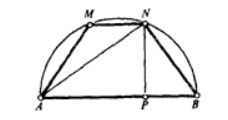
\includegraphics[scale=1.2]{pic1.png}
    Рис.1.
    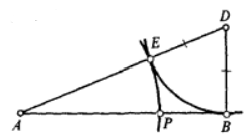
\includegraphics[scale=1.2]{pic2.png}
    Рис.2.
    
    \vspace{6pt}
    \Huge \bf 24
    
    
    \end{minipage} 
    \hspace{0.8cm}
    \begin{minipage}{0.75\textwidth}
    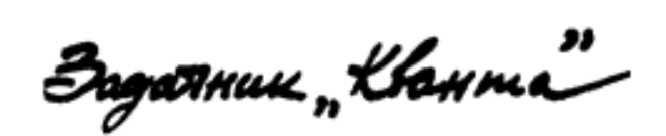
\includegraphics{header.png}
    
    \vspace{6pt}
    % \begin{flushright}
    %     \textls{Таблица}  \par \vspace{5pt}
    % \end{flushright}
    \hspace*{\hfill} \textls{Таблица}  \par \vspace{5pt}
    
        {\begin{tabular}{|m{0.9in}|>{\centering\arraybackslash}m{0.85in}|>{\centering\arraybackslash}m{0.9in}|>{\centering\arraybackslash}m{0.5in}|>{\vspace{2pt}\centering\arraybackslash}m{0.45in}|}
    
        
        \hline
    
         \centering Матириал & Q, Ом мм$^2$/м (при 20 $^\circ C$) &  $\alpha$, град$^{-1}$ \par (при 20 $^\circ C$) &  Плот- ность, г/см$^3$ & Темпе- ратура плавления,  {$^\circ C$} \\
         \hline
         \rowcolor{green}
           Алюминий &  0,032 &  0,038 &  2,6$-$2,8 &  660 \\
         \rowcolor{yellow}
        Бронза & 0,12 & 0,004 & 7,4$-$8,8 & 1000 \\
         \rowcolor{green}
        Вольфрам & 0,055 & 0,0051 & 19,0 & 3387 \\
         \rowcolor{yellow}
        Золото & 0,024 & 0,0039 & 19,3 & 1063 \\
         \rowcolor{green}
        Кобальт & 0,097 & 0,0033 & 8,8 & 1490 \\
         \rowcolor{yellow}
        Латунь & 0,06$-$0,09 & 0,001$-$0,007 & 8,4$-$8,7 & 900 \\
         \rowcolor{green}
        Медь & 0,017 & 0,0043 & 8,6$-9,0$ & 1083 \\
         \rowcolor{yellow}
        Молибден & 0,048 & 0,0050 & 10,2 & 2622 \\
         \rowcolor{green}
        Никель & 0,11 & 0,0027 & 8,8 & 1452 \\
         \rowcolor{yellow}
        Олово & 0,11 & 0,0044 & 7,3 & 232 \\
         \rowcolor{green}
        Платина & 0,09 & 0,0038 & 21,4 & 1773 \\
         \rowcolor{yellow}
        Свинец & 0,21 & 0,0042 & 11,3 & 327 \\
         \rowcolor{green}
        Серебро & 0,016 & 0,0040 & 10,5 & 961 \\
         \rowcolor{yellow}
        Сталь & 0,199 & 0,0016$-$0,0042 & 7,5$-$7,9 & 1500 \\
         \rowcolor{green}
        Хром & 0,027 & 0,0042 & 6,7 & 1700 \\
         \rowcolor{yellow}
        Цинк & 0,060 & 0,0039 & 6,8$-$7,1 & 419 \\ \hline
    
    \end{tabular}}
    \hspace*{\fill}{}
    \vspace{6pt}
    
    \textbf{Ф1307.} Квант электромагнитного излучения испытывает рассеяние на покоящемся эелктроне (так называемый Комптон-эффект). При этом рассеянный квант изменяет частоту, а электрон получает импульс отдачи \textit{p}. Определите, под какими углами по отношению к направлению падающего излучения может двигаться электрон с данным импульсом. Считайте, что скорость электрона существенно меньше, чем скорость света.    
    
    % \begin{flushright}
    %      \textit{Ю Самарский}
    %  \end{flushright}
     \hspace*{\fill} \textit{Ю Самарский}
    
    \section*{\textbf{Решения задач}}
    \textbf{M1271$-$M1275, Ф1283$-$Ф1287}
    \vspace{6pt} \\
    Пусть \textit{AMNB} $-$ искомая трапеция и \textit{NP} $-$ ее высота.
    Так как трапеция вписана в окружность, то ее боковые стороны равны. Но трапеция является и описанной, поэтому каждая из ее боковых сторон равняется полусумме оснований, т.е. отрезку \textit{AP}. Из подобия треугольников \textit{ANB} и \textit{NPB} (рис. 1) следует равенство 
    \begin{equation*}
    AP^2=NB^2=AB\cdot BP
    \tag{\textbf{$*$}}
    \end{equation*}
    % \[AP^2=NB^2=AB\cdot BP\]
    % \hspace*{\fill} \textbf{($*$)}
        
    т.е. точка \textit{P} делит отрезок \textit{AB}, как говорят, <<в крайнем и среднем отношении>>. Построение такой точки можно выполнить следующим образом: восставим к \textit{AB} перпендикуляр \textit{BD}$=\frac{1}{2}AB$ (рис. 2), отложим не отрезке \textit{AD} отрезок \textit{DE$=$DB}, а на \textit{AB} отрезок \textit{AP$=$AE}. Если \textit{AB$=$}2, то, как легко проверить, $AP=\sqrt{5}-1$ и для точки \textit{P} выполнено соотношение \textbf{($*$)}. \par
    \hspace{10pt} Затем можно, восстановив перпендикуляр \textit{PN} в точке \textit{P} к отрезку \textit{AB} до пересечения с полуокружностью, построить искомую равнобочную трапецию \textit{AMNB} и доказать (используя подобие треугольников), что ее боковая сторона равна \textit{AP}, т.е. полусумме оснований, следовательно, она описанная.
    
    
    \end{minipage}
    
    \newpage
    
    \begin{minipage}{0.25\textwidth}
    \vspace{1.3cm}
    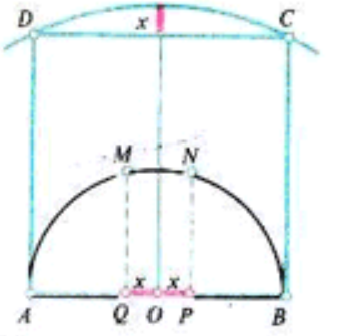
\includegraphics[scale=0.8]{pic3}
    \it Рис.3. \par
    \vspace{0.6cm}
    \hspace*{\fill} 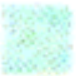
\includegraphics[scale=0.8]{cube.png} \par
    \it \textbf{M1272}. Докажите, что для любых n положительных чисел $a_1, a_2, ..., a_n$, сумма которых равна 1, выполнено неравенство 
    \vspace{3pt}
    \hspace*{\fill} $(1/a^2_1-1)(1/a^2_2-1)...$\par \hspace*{\fill} $...(1/a^2_n-1)\geq(n^2-1)^n$.
    
    \vspace{2.8cm}
    \hspace*{\fill} 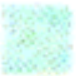
\includegraphics[scale=0.8]{cube.png}
    \end{minipage}
    \hspace{0.8cm}
    \begin{minipage}{0.75\textwidth}
    % \vspace{2cm}
        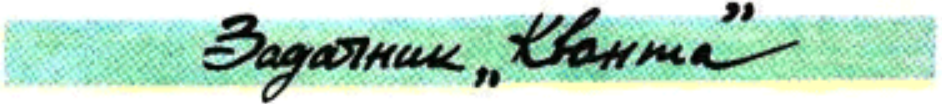
\includegraphics[scale=0.90]{header2.png} \par
    \vspace{8pt}
    \hspace{10pt} 
    Еще один из возможных способов построения трапеции основан на идее, изложенной в статье <<Правильные многогранники и повороты>> (<<Квант>> \textnumero 10, 1989). Строим квадрат \textit{ABCD}, проводим через его вершины \textit{C} и \texti{D} дугу окружности с центром в точке \textit{O}$-$середине стороны \textit{AB} (рис. 3). Восставим из точки \textit{O} перпендикуляр к \textit{AB}, его отрезок \textit{x} (он равен $\sqrt{5}-2$) между квадратом и построенной дугой окружности отложим от точки \textit{O} влево и вправо по отрезку \textit{AB}. Полученные точки \textit{Q} и \textit{P}$-$проекции вершин \textit{M} и \textit{N} трапеции на основание \textit{AB}. 
    
    % \begin{flushright}
    % \textit{В. Сендеров}
    % \end{flushright}
    \hspace*{\fill} \textit{В. Сендеров} 
    
    \vspace{0.6cm}
    
    Если сближать два числа \textit{u, v} $(0<u<v<1)$ так, чтобы их сумма оставалась постоянной, то произведение $uv=(u+v)^2/4-(u-v)^2/4$ увеличивается, а произведение $(1/u^2-1)(1/v^2-1)=(1-u^2-v^2+u^2v^2)/u^2v^2=(1-(u+v^2)/u^2v^2+2uv+1$ уменьшается. Из \textit{n} чисел с суммой 1, среди которых не все равны $1/n$, найдется число \textit{u}, меньшее $1/n$, и число \textit{v}, большее $1/n$ (подобное соображение играло ключевую роль в <<самом коротком доказательстве теоремы Коши>>, см. статью Ю. П. Соловьева в <<Кванте>> \textnumero 3 за этот год). Будем сближать \textit{u} и \textit{v}, сохраняя сумму до тех пор, пока одно из них не станет равным $1/n$; при этом произведение $P=(1/a^2_1-1)\times...\times(1/a^2_n-1)$ будет уменьшаться. Если в полученном наборе еще не все числа равны $1/n$, можно повторить эту процедуру с другой парой чисел и поступать так до тех пор, пока все числа не станут равны $1/n$; при этом \textit{P} станет равным $(n^2-1)^n$. Тем самым, первоначально произведение \textit{P} было не меньше этой величины.
    
    % \begin{flushright}
    % \textit{Л. Курляндчик}
    % \end{flushright}
    \hspace*{\fill} \textit{Л. Курляндчик}
    
    $f(x)=\sum\limits^{k=\infty}_{k=0}k\cdot\sqrt[3]{\frac{1}{k+x}}$
    \end{minipage}
    % \end{document}